\documentclass[11pt]{article}
\usepackage[utf8]{inputenc}
\usepackage{fancyhdr}
\usepackage{diagbox}
\usepackage[english]{babel}
\usepackage{latexsym}
\usepackage{graphicx}
\usepackage{array}
\usepackage{amsmath}
\usepackage{amssymb}
\usepackage{mathtools}
\usepackage{algorithmicx}
\usepackage{algpseudocode}
\renewcommand{\baselinestretch}{1.0}
\usepackage[letterpaper, margin=0.75in]{geometry}
\DeclarePairedDelimiter{\ceil}{\lceil}{\rceil}
\pagestyle{fancy}
\lhead{}
\rhead{Yu Mi, yxm319. Algorithm HW5}
\renewcommand{\thesubsection}{\alph{subsection}}
\def\QEDclosed{\mbox{\rule[0pt]{1.3ex}{1.3ex}}}
\begin{document}
	\title{Homework 5 for EECS 340}
	\author{Yu Mi,yxm319}
	\maketitle
\section{Warm-Up: Applying Dynamic Programming Algorithms}
Use the dynamic programming algorithms given in class to solve the following problems. Show your work.
\subsection{Coins in a Line}
Suppose that in an instance of he coins-in-a-line game the coins have the following values in the line:
$$(9,1,7,3,2,8,9,3)$$
What is the maximum that the first player, Alice,can win, assuming that the second player, Bob, play optimally?

\noindent \emph{Answer} :
To solve this problem, let's define $M_{i,j}$ to be the maximum value of coins taken by Alice, for coins numbered $i$ to $j$, and Bob plays optimally. Therefore, the optimal value for Alice is determined by $M_{1,8}$.

Assume the values of each coin are in the array $V[i]$. The principle of Alice to choose is list as follow:

\begin{enumerate}
	\item If $j=i+1$, Alice should pick up the larger one in $V[i]$ and $V[j]$;
	\item Otherwise, if Alice chooses coin $i$, then she gets a total value of $$\min\{M_{i+1,j-1},M_{i+2,j}\}+V[i];$$
	\item Otherwise, if Alice chooses coin $j$, then she gets a total value of $$\min\{M_{i,j-2},M_{i+1,j-1}\}+V[j].$$
\end{enumerate}

To sum up, for $j>i+1$, we have $$M_{i,j}=\max\{\min\{M_{i+1,j-1},M_{i+2,j}\}+V[i],\min\{M_{i,j-2},M_{i+1,j-1}\}+V[j]\}$$

As to the initial situation, we have $M_{i,i+1}=\max\{V[i],V[i+1]\},i\leq(n-1)$, thus, we can fill out the table for $M_{i,j}$ as shown in Table.\ref{tab:tab1}.
\begin{table}[hbp]
	\centering
	\tiny
	\caption{Values for $M$}
	\begin{tabular}{c|c|c|c|c|c|c|c|c}
		\hline 
		\hline
		\diagbox{$i$}{$j$}	&1	&2	&3	&4	&5	&6	&7	&8	\\
		\hline
		1	&9	&9	&10	&16	&13	&18	&21	&27	\\
		\hline
		2	&0	&1	&7	&4	&9	&12	&18	&15	\\
		\hline
		3	&0	&0	&7	&7	&9	&11	&18	&18	\\
		\hline
		4	&0	&0	&0	&3	&3	&10	&12	&14	\\
		\hline
		5	&0	&0	&0	&0	&2	&8	&11	&11	\\
		\hline
		6	&0	&0	&0	&0	&0	&8	&9	&11	\\
		\hline
		7	&0	&0	&0	&0	&0	&0	&9	&9	\\
		\hline
		8	&0	&0	&0	&0	&0	&0	&0	&3	\\
		\hline
		\hline
	\end{tabular}
	\label{tab:tab1}
\end{table}

Thus, we can conclude Alice can get the value of $27$ to win.
\subsection{0-1 Knapsack}\label{NEED TO TRACEBACK}
Let $S=\{a,b,c,d,e,f,g\}$ be a collection of objects with benefit-weight values, $a:(12,4), b:(10,6), c:(8,5), d:(11,7), e:(14,3),f:(7,1), g:(9:6)$. What is the optional solution to the 0-1 knapsack problem for $S$ assuming we have a sack that can hold with total weight $18$? Show your work.

\noindent \emph{Answer}: Let's define $B[k,w]$ as the maximum total value of a subset of $S_k$ from among all those subsets having weight at most $w$. As initial, we have $B[0,w]$ for each $w\leq W$, then we have the following relationship:
$$
	B[k,w]=\left\{
		\begin{aligned}
		&B[k-1,w],& \text{if } w_k>w\\
		&\max\{B[k-1,w],B[k-1,w-w_k]+b_k\}, &\text{else}.
		\end{aligned}
	\right.
$$

Following the method mentioned above, we have the table for $B[7,w]$ shown as Table.\ref{tab:tab2}
\begin{table}[!hbp]
	\centering
	\tiny
	\caption{Values for $B[7,w]$}
	\begin{tabular}{c|c|c|c|c|c|c|c|c|c|c|c|c|c|c|c|c|c|c}
		\hline 
		\hline
		$w$	&1	&2	&3	&4	&5	&6	&7	&8	&9	&10	&11	&12	&13	&14	&15	&16	&17	&18\\
		\hline
	$B[7,w]$&7	&7	&14	&21	&21	&21	&26	&33	&33	&33	&33	&34	&41	&43	&44	&44	&44	&44\\
		\hline
		\hline
	\end{tabular}
	\label{tab:tab2}
\end{table}

As is shown above, we can conclude that the maximum benefit we can have is $44$, which contains item $(12,4), (11,7), (14,3), (7,1)$.
\subsection{Telescope Scheduling Redux}
Suppose we are given a set of telescope observation requests, specified by triples of $(s_i,f_i,b_i)$, defining the start times, finish times, and benefits of each observation request as $$L=\{(1, 2, 5), (1, 3, 4), (2, 4, 7), (3, 5, 2), (1, 6, 3), (4, 7, 5), (6, 8, 7), (7, 9, 4)\}.$$
Solve the telescope scheduling problem for this set of observation requests.

\noindent \emph{Answer}: As is discussed in former homeworks, we define $\text{pred}(i)$ as the predecessor of each request $i$, which has the value of following:$$\text{pred}(i)=\{0,0,1,2,0,3,5,6\}.$$
Therefore, we can then define $B[i]$ to be the maximum benefit can be achieved with the first $i$ requests. The recursive definition would be: $$B_i=\max\{B_{i-1},B_{\text{pred}(i)}+b_i\}.$$

Thus, the $B[i]$ will have the value as shown in Table.\ref{tab:tab3}.
	\begin{table}[!hbp]
	\centering
	\tiny
	\caption{$B_i$ values}
	\begin{tabular}{c|c|c|c|c|c|c|c|c|c}
		\hline 
		\hline
		$i$  &0	&1	&2	&3	&4	&5	&6	&7	&8\\
		\hline
		$B_i$&0	&5	&4	&12	&6	&3	&17	&13	&21\\
		\hline
		\hline
	\end{tabular}
	\label{tab:tab3}
\end{table}

As is shown above, we can have the maximum benefit of $21$, the corresponding tasks are: $$(1,2,5), (2,4,7),(4,7,5),(7,9,4).$$
\section{Warm-Up: Applying Greedy Algorithms}
Use the greedy algorithms given in class to solve the following problems. Show your work.
\subsection{Fractional Knapsack}
Let $S=\{a,b,c,d,e,f,g\}$ be a collection of objects with benefit-weight values, $a:(12,4),b:(10,6),c:(8,5),d:(11,7),e:(14,3),f:(7,1),g:(9,6)$. What is an optimal solution to the fractional knapsack problem for $S$ assuming we have a sack that can hold objects with total weight $18$? Show your work.
\noindent \emph{Answer}: Since this question asks for fractional knapsack, we can calculate the benefit-per-weight values as follows: $a:3, b:1.667,c:1.4,d:1.571,e:4.667,f:7,g:1.5$. Thus we can pick up the objects according to their benefit-per-weight. The weight for objects to take is :$f:1,e:3,a:4,b:6,d:4$, the total value would be $7+14+12+10+4\times \frac{11}{7}=49.286$.
\subsection{Task Scheduling}
Suppose we are given a set of tasks specified by pairs of the start times and finish time as $$T=\{(1,2),(1,3),(1,4),(2,5),(3,7),(4,9),(5,6),(6,8),(7,9)\}.$$ Solve the task scheduling problem for this set of tasks.
\noindent \emph{Answer}: To solve the task scheduling problem with greedy algorithm, we can append the new tasks right behind the end of a prior task. Thus we have:
\begin{enumerate}
	\item $\{(1,2),(2,5),(5,6),(6,8)\}$
	\item $\{(1,3),(3,7),(7,9)\}$
	\item $\{(1,4),(4,9)\}$
\end{enumerate}
All the tasks can be solved by three workers.
\section{Warm-Up: Coins in a Line and the Failings of Greed}
Show that, in the coins-in-a-line game, a greedy-denial strategy of having the first player, Alice, always choose the available coin that minimizes the maximum value of the coin available to Bob will not necessarily result in an optimal solution for her.

\noindent \emph{Answer}: When we have the coins in the line are $(1,9,8,7,1)$, Alice may take the leftmost $(1)$ in the first place, Bob will take $(7)$, Alice then take $(8)$, Bob then take $(9)$, Alice will finally take $(1)$. Thus Bob will have a total value of $7+9=16$, and Alice will have $10$. 
\section{The Cleveland Pothole Problem}
\noindent \emph{Answer}: Since each of the metal plates can cover a length of $24'$, we can first sort the potholes in a increasing order and then group the potholes that can be covered by a single plate. The algorithm is shown as follow:
\begin{algorithmic}
	\State \textbf{Algorithm} CoverHoles($S$)
	\State \textbf{Input}: $n$ positions of the potholes.
	\State \textbf{Output}: The number of plates needed.
	\State $P\gets$ sorted $S$ in increasing order
	\State $Plates \gets 0, Previous\gets-\infty$
	\For{$i\gets1$ to $n$}
		\If{$Previous + 24<P[i]$}\Comment This hole cannot be covered by the previous plate
			\State $Plates \gets Plates + 1$
			\State $Previous \gets P[i]$
		\EndIf
	\EndFor
	\State \Return $Plates$
\end{algorithmic}
\section{Zombie Apocalypse: Cooking Edition}
\noindent \emph{Answer}: In mathematics, the \textbf{rearrangement inequality} states that $$x_ny_1 + \cdots + x_1y_n \le x_{\sigma (1)}y_1 + \cdots + x_{\sigma (n)}y_n \le x_1y_1 + \cdots + x_ny_n$$ for every choice of real numbers $$x_1\le\cdots\le x_n\quad\text{and}\quad y_1\le\cdots\le y_n.$$

The proof is as follows:

Observe first that $x_1 > x_2\text{ and } y_1 > y_2$, implies $(x_1-x_2)(y_1-y_2) > 0  \text{ or } x_1y_1 + x_2y_2 > x_2y_1 + x_1y_2,$, hence the result is true if $n = 2$. 

Assume it is true at rank $n-1$, and let $x_1>\cdots>x_n,\text{ and } y_1>\cdots>y_n.$ Choose a permutation $\sigma$ for which the arrangement gives rise a maximal result.

If $\sigma(n)$ were different from $n$, say $\sigma(n) = k$, there would exist $j<n$ such that $\sigma(j) = n.$ 

But $x_n > x_k \text{ and } y_n > y_k,\text{ hence } x_ny_n + x_ky_k > x_ky_n + x_ny_k$, by what has just been proved. Consequently, it would follow that the permutation $\tau$ coinciding with $\sigma$, except at $j$ and $n$, where $\tau(j) = k \text{ and } \tau(n) = n$, gives rise a better result. This contradicts the choice of $\sigma$. Hence $\sigma(n) = n$, and from the induction hypothesis, $\sigma(i) = i$ for every $i < n$.

The same proof holds if one replace strict inequalities by non strict ones. \QEDclosed

According to this, we can simply select the largest $c_i$ to pair with largest $b_i$, then the second largest pair and so forth. The algorithm is described as follow:
\begin{algorithmic}
	\State \textbf{Algorithm} Pairing($C,B$)
	\State \textbf{Input}: a list of calories $C$ and a list of benefits $B$, both have a size of $n$.
	\State \textbf{Output}: The maximum total benefit.
	\State $C'\gets$ sorted $C$ in increasing order
	\State $B'\gets$ sorted $B$ in increasing order
	\State $sum\gets0$
	\For{$i\gets 1$ to $n$}
		\State $sum\gets C'[i]\times B'[i]$
	\EndFor
	\State \Return $sum$
\end{algorithmic}
\section{Checker-Sum Redux}

\noindent \emph{Answer}: Since the checker-sum can be computed based on the former checker-sum, we can then use dynamic programming to calculate these latter values.

Specifically, we have:
\begin{equation*}
\begin{aligned}
	\text{checker-sum}(A)_{i,j}&=(-1)^{i+j}\sum_{k=1}^{i}\sum_{l=1}^{j}(-1)^{k+l}A_{k,l}\\
	&=(-1)^{i+j}\sum_{k=1}^{i-1}\sum_{l=1}^{j-1}(-1)^{k+l}A_{k,l}+(-1)^{i+j}\sum_{l=1}^{j-1}(-1)^{i+l}A_{i,l}+(-1)^{i+j}\sum_{k=1}^{i-1}(-1)^{k+j}A_{k,j}+(-1)^{i+j}A_{i,j}\\
	&=\text{checker-sum}(A)_{i-1,j-1}-(\text{checker-sum}(A)_{i-1,j}-\text{checker-sum}(A)_{i-1,j-1})-\\
	&\text{\quad}(\text{checker-sum}(A)_{i,j-1}-\text{checker-sum}(A)_{i-1,j-1})+(-1)^{i+j}A_{i,j}\\
	&=3\times\text{checker-sum}(A)_{i-1,j-1} - \text{checker-sum}(A)_{i,j-1} - \text{checker-sum}(A)_{i-1,j} + (-1)^{i+j}A_{i,j}
\end{aligned}
\end{equation*}
Thus, we have the algorithm:
\begin{algorithmic}
	\State \textbf{Algorithm} Checker-Sum($A$)
	\State \textbf{Input}: a matrix $A\in \mathbb{R}^{n\times n}$
	\State \textbf{Output}: The checker-sum of A.
	\State $Sum \gets$ an all-zero $n\times n$ matrix \Comment Includes initial conditions: all sum are zero
	\For{$i\gets1$ to $n$}
		\For{$j\gets1$ to $n$}
			\State $Sum[i,j] \gets 3\times Sum[i-1,j-1]-Sum[i,j-1]-Sum[i-1,j]+(-1)^{i+j} A_{i,j}$
		\EndFor
	\EndFor
	\State \Return $Sum$
\end{algorithmic}
\section{On The Grid}
\noindent \emph{Answer}: Since each of the input $n,m$ will be related to the direct next indice of $n,m$ we can do dynamic programming from the first one to the last one:
\begin{algorithmic}
	\State \textbf{Algorithm} F'($L,n,m$)
	\State \textbf{Input}: the topological ordering $L$, and the dimensions $n,m$.
	\State \textbf{Output}: The same value of F($n,m$)
	\State $Results \gets$ an empty $n\times m$ matrix 
	\For{$k\gets 1$ to $L.length$}
		\State $i\gets L[k,0]$\Comment get the $k$-th element of L
		\State $j\gets L[k,1]$
		\If {$Test(i,j)$}
			\State $Results[i,j].append(Base(i,j))$
		\Else
			\State $I\gets\text{NextIndices}(i,j)$
			\For{$(i,j)\in I$}
				\State $Results[i,j].append(\text{Combiner}(Results[i,j]))$
			\EndFor
		\EndIf
	\EndFor
	\State \Return $Results[n,m]$
\end{algorithmic}
\section{A State of Balance}
Suppose we are given a collection $A=\{a_1,a_2,...,a_n\}$ of $n$ positive integers and add up to $N$. Design an $O(nN)$-time algorithm for determining whether there is a subset $B\subset A$ such that $\sum_{a_i\in B}a_i=\sum_{a_i\in A-B}a_i$.
\noindent \emph{Answer}: We can use dynamic programming(DP) to solve this problem. First, we define our DP table $Table[i,j]$ where $0\leq i\leq n$ and $0\leq j\leq N$which picks value from between $True$ and $False$ saying that there is a subset of items in $A_i=\{a_1,a_2,...,a_n\}$ that adds to exactly $j$. Thus our solution will be $Table [n,N/2]$.

As to the initial conditions, $Table[0,0]=1$, and for any $i>0$, $Table[0,i]=0$ and $Table[i,0]=1$(picking nothing). For any $i\geq1$ and $j\geq1$, we have: $$Table[i,j]= \max\{Table[i-1,j],Table[i-1,j-a_i]\}$$ when $j>=a_i$. Such that the running time would be $O(nN)$. The algorithm is shown as follow:
\begin{algorithmic}
	\State \textbf{Algorithm} CanBalance($A,n,N$)
	\State \textbf{Input}: A list of positive number $A$, and its length $n$, its sum $N$
	\State \textbf{Output}: Whether there is a $B$ that $\sum_{a_i\in B}a_i=\sum_{a_i\in A-B}a_i$.
	\If{$N$ is odd number}
		\State \Return $False$ \Comment When $N$ is odd, there can't be possible balance.
	\EndIf
	\State $Table\gets$ an $n\times N$ matrix with default value all $False$.
	\State $Table[:,0]\gets True$\Comment Assign all $Table[i,0]=1$
	\For{$j\gets 1$ to $N$}
		\For{$i\gets 1$ to $n$}
			\If{$j\geq a_i$}
				\State $Table[i,j]\gets Table[i-1,j] + Table[i-1,j-a_i]$ \Comment Logical plus, return $True$ or $False$
			\Else
				\State $Table[i,j]\gets Table[i-1,j]$
			\EndIf
		\EndFor
	\EndFor
	\State \Return $Table[n,N/2]$
\end{algorithmic}
\section{Monotonically Decreasing Subsequences}
Describe an $O(n^2)$ algorithm to find the length of the longest monotonically (strictly) decreasing subsequence(s) of $n$ integers. For example, given the sequence $(2,4,1,3) (n=4)$, the decreasing subsequences are $(4,1),(2,1),(4,3),(2),(4),(1),\and (3)$, so your algorithm should return $2$ in this case.

\noindent \emph{Answer}: To do this, we can define our DP table as $B[i]$, which stands for the longest decreasing subsequences from $i$ to $n$. Thus, for each of $i$, we only need to find if there is any $B[j], j\in [i,n]$ which $B[j]$is smaller than $B[i]$, then $B[i] = \max\{B[j]+1\}$.

As to the initial condition, we only need to set all the $B[i]$ to $1$, since each of the elements in the list can be a single subsequence with length $1$. The algorithm can be shown as follows:

\begin{algorithmic}
	\State \textbf{Algorithm} MDS($S,n$)
	\State \textbf{Input}: A list of positive number $S$, and its length $n$.
	\State \textbf{Output}: The length of the longest monotonically decreasing subsequence.
	\State $B\gets$ a list with size $n$ and all values initially set to $1$
	\State $max\gets1$\Comment Marks the max length
	\For{$i \gets n$ to $1$}
		\For{$j\gets i$ to $n$}
			\If{$S[i]>S[j]$ and $B[j]+1>B[i]$}
				\State $B[i]\gets B[j]+1$
			\EndIf
		\EndFor
		\If{$max<B[i]$}
			\State $max\gets B[i]$
		\EndIf
	\EndFor
	\State \Return $max$
\end{algorithmic}
\section{Let's Do the Time Warp Again}
Speech recognition systems need to match audio streams that represent the same words spoken at different speeds. Suppose, therefore, that you are given two sequences of numbers,$X=(x_1,x_2,...,x_n)$ and $Y=(y_1,y_2,...,y_m)$, representing two different audio streams that need to be matched. A mapping between $X$ and $Y$ is a list, $M$, of distinct pairs, $(i,j)$, that is ordered lexicographically, such that, for each $i\in [1,n]$, there is at least one pair, $(i,j)$, in $M$, and for each $j\in[1,m]$, there is a least one pair, $(i,j)$, in $M$.  Such a mapping is monotonic if, for any $(i,j)$ and $(k,l)$ in $M$, with $(i,j)$ coming before $(k,l)$ in $M$, we have $i\leq k$ and $j\leq l$. For example, given $$X=(3,9,9,5) \text{ and } Y=(3,3,9,5,5),$$ one possible monotonic mapping between $X$ and $Y$ would be $$M=[(1,1),(1,2),(2,3),(3,3),(4,4),(4,5)].$$ The dynamic time warping problem is to find a monotonic mapping, $M$, between $X$ and $Y$, that minimizes the distance $D(X,Y)$, between $X$ and $Y$, subject to $M$, which is defined as $$D(X,Y)=\sum_{(i,j)\in M}|x_i-y_i|,$$ where this minimization is taken over all possible monotonic mappings between $X$ and $Y$. For instance, in the example $X$,$Y$, and $M$, given above, we have $D(X,Y)=0$. Describe an efficient algorithm for solving the dynamic time warping problem. What is the running time of your algorithm?
\noindent \emph{Answer}: Since each of the $x_i$ and $y_i$ can be computed from $1$ to $n$ in an incremental way and only have $3$ possibilities of transform: insertion, deletion and match, we can simply select the smallest way of cost to determine the optimal $D(X,Y)$. As to the initial condition, we can simply set all the boundaries to $\infty$. The algorithm is shown as follow:
\begin{algorithmic}
	\State \textbf{Algorithm} DTWDistance($X,Y,n,m$)
	\State \textbf{Input}: Array $X\and Y$ with size $n\and m$
	\State \textbf{Output}: The smallest possible $D(X,Y)$
	\State $DTW\gets$ an $n\times m$ matrix with initial value all zero
	\State $DTW[:,0]\gets \infty$\Comment Set all boundary cost to $\infty$
	\State $DTW[0,:]\gets \infty$\Comment Set all boundary cost to $\infty$
	\For{$i\gets 1$ to $n$}
		\For {$j\gets 1$ to $m$}
			\State $cost\gets |X[i]-Y[j]|$
			\State $DTW\gets cost + \min(DTW[i-1,j],DTW[i,j-1],DTW[i-1,j-1])$
		\EndFor
	\EndFor
	\State \Return $DTW[n,m]$
\end{algorithmic}
\section{EECS454 only}
\subsection{R-17.9}
Given $B=(x_1+\overline{x_2}+x_3)\cdot(x_4+x_5+\overline{x_6})\cdot(x_1+\overline{x_4}+\overline{x_5})\cdot(x_3+x_4+x_6)$, draw the instance of VERTEX-COVER that is constructed by the reduction from 3SAT of the Boolean formula $B$.

\noindent \emph{Answer}: The figure is shown as Fig.\ref{fig:fig1}:
\begin{figure}[!h]
	\centering
	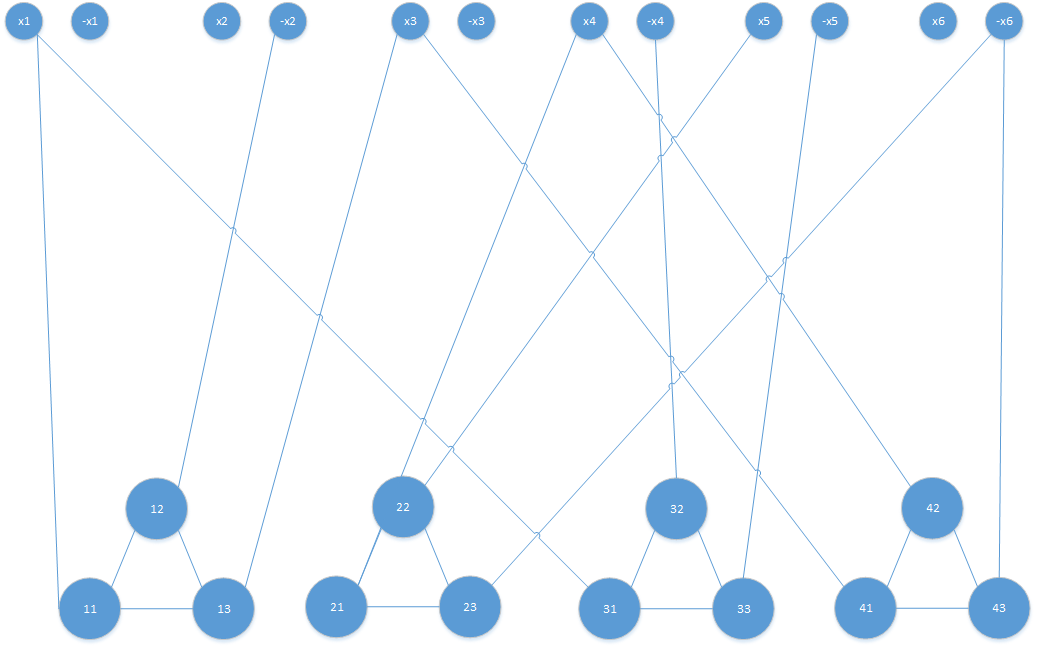
\includegraphics[width=0.9\textwidth]{Figure/R-179.png}
	\caption{Instance of VERTEX-COVER($x_4$ is connected to 21 and 42)}
	\label{fig:fig1}
\end{figure}
\subsection{R-17.10}
Draw an example of a graph with $10$ vertices and $15$ edges that has a vertex cover of size $2$.

\noindent \emph{Answer}: The figure is shown as Fig.\ref{fig:fig2}:
\begin{figure}[!h]
	\centering
	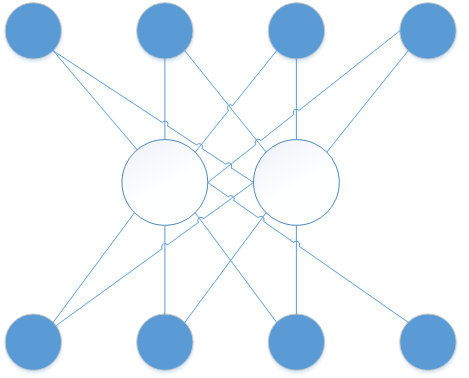
\includegraphics[width=0.6\textwidth]{Figure/R-1710.png}
	\caption{Possible graph}
	\label{fig:fig2}
\end{figure}

One vertex cover is the set which contains only the two white nodes in the center.
\subsection{R-17.12}
Professor Amongus has just designed an algorithm that can take any graph G with n vertices and determine in $O(n^k)$ time whether $G$ contains a clique of size $k$. Does Professor Amongus deserve the Turing Award for having just shown that \textbf{P = NP}? Why or why not?

\noindent \emph{Answer}: Determining whether a graph has a clique of size $k$ in polynomial time can only break its \textbf{NP}-completeness, hence it does not prove \textbf{P = NP}.
\subsection{C-17.10}
Define INDEPENDENT-SET as the problem that takes a graph $G$ and an integer $k$ and asks whether $G$ contains an independent set of vertices of size $k$. That is, $G$ contains a set $I$ of vertices of size $k$ such that, for any $v$ and $w$ in $I$, there is no edge $(v,w)$ in $G$. Show that INDEPENDENT-SET is \textbf{NP}-complete.
\noindent \emph{Answer}: Assume $G$ is a instance of CLIQUE, which means there exists a CLIQUE $C$ of size $k$ in $G$. Thus, for any $u,v\in C, (u,v)\in E$. Thus, $(u,v)\not\in E^c$. Thus, the vertices in $C$ form an INDEPENDENT-SET in $G^c$, and $G^c$ is a instance of INDEPENDENT-SET. Thus, we can reduce INDEPENDENT-SET problem to a CLIQUE problem, which is \textbf{NP}-complete, which means INDEPENDENT-SET is also \textbf{NP}-complete.
\end{document}